\subsection{Programmable Privacy}

Programmability The privacy platform has two main features (1)It supports private 
transactions, not only private transactions. Similar to Zcash \cite{website:Zcash}, users can still 
choose the transaction type, public transaction or private transaction independently; 
(2)Support Programmability, you can deploy any smart contract, public contract or 
private contract, depending on the needs of the project party. Compared with Specific 
Privacy, the main difference is the logic of state transition in Note, from specific 
calculation to arbitrary calculation logic. Figure \ref{fig:Difference between Specific Privacy and Programmable Privacy} simply shows the difference 
between the two.
\begin{figure}[!ht]
    \centering
    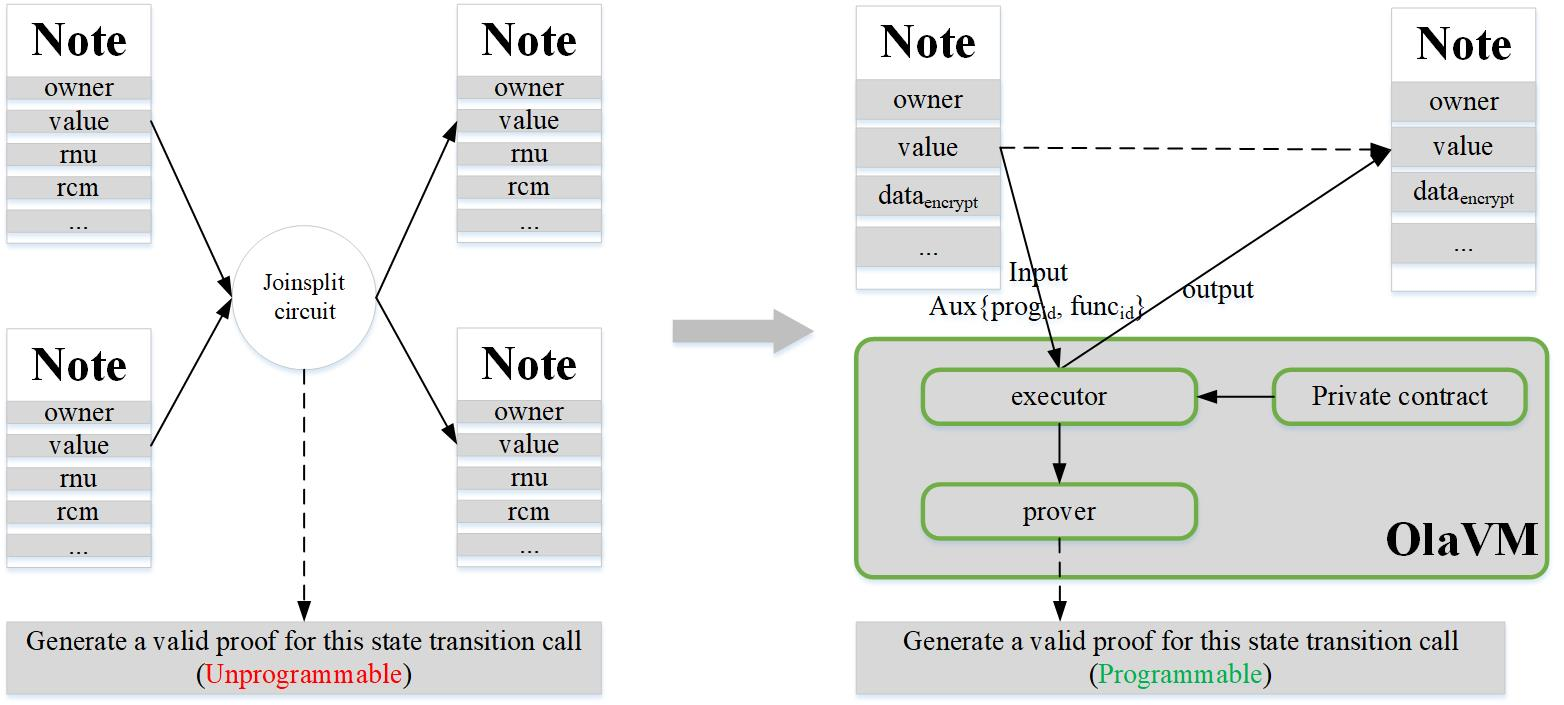
\includegraphics[width=0.8\textwidth]{Difference between Specific Privacy and Programmable Privacy.jpg}
    \caption{Difference between Specific Privacy and Programmable Privacy}
    \label{fig:Difference between Specific Privacy and Programmable Privacy}
\end{figure}

The current projects focusing on programmable privacy are Aleo \cite{website:Aleo} and Aztec \cite{website:Aztec}. Aleo \cite{website:Aleo} is a 
privacy public chain, from BTC \cite{website:BTC} to Ethereum \cite{website:Ethereum} to Zcash \cite{website:Zcash} to Aleo \cite{website:Aleo}. It makes up for 
the fact that programmability and privacy cannot coexist at the Layer1 level. 
It has reached the testnet stage and supports developers to deploy privacy contracts; 
Aztec \cite{website:Aztec} focuses on doing Layer2 programmable privacy for Ethereum \cite{website:Ethereum} , a project 
called Aztec3 \cite{website:Aztec3}, is still in development.

There are often two ways to achieve programmability, one is to customize Domain Specific Language (DSL), such as Circom \cite{website:Circom} , Pil \cite{website:Pil}, Noir \cite{website:Noir}, etc.; the other is Smart Contract Language (SCL), 
such as Cairo1.0 \cite{website:Cairo1.0}, Solidity \cite{website:Solidity}, Ola lang \cite{website:Ola-lang} and so on. The main difference is that SCL is defined in the Instruction Set Architecture (ISA) on a General Purpose Language (GPL), compared to DSL, 
with higher abstraction, but also more suitable for writing complex business logic; and DSL abstraction is lower, more suitable for some simple computational expression. 
Take Polygon Hermez's \cite{website:Polygon-Hermez} Pil \cite{website:Pil} language as an example, you can directly use it to define a simple micro-op, such as `A * B + C`, or `A * B * C + D` and other simple combinations. 
Table \ref{table:Difference between DSL and SCL} briefly shows some of the differences between DSL and SCL.

\begin{table}[!ht]
    \centering
    \begin{tabular}{|l|l|l|l|l|l|}
    \hline
        \emph{Type} & \emph{Abstraction} & \emph{Process} & \emph{Difficulty} & \emph{Examples} & \emph{Notes} \\ \hline
        DSL & low & program -> arith-ops -> ops gadgets & normal & \makecell{circom \\ noir \\ cairo} & \makecell{1. semantic analysis \\ 2. codeGen optimization} \\
        \makecell{SCL \\ (ISA/VM)} & high & program -> bytecodes -> cpu circuit & hard & \makecell{solidity \\ cairo1.0 \\ ola lang} & \makecell{1. need a compiler \\2. re-use LLVM framework} \\
    \end{tabular}
    \caption{Difference between DSL and SCL}
    \label{table:Difference between DSL and SCL}
\end{table}

For DSL, you may need to predefine some commonly used operators, each corresponding to a circuit, called a Gadget \cite{website:Gadget}; you can use these operators to combine any desired calculation logic and 
encapsulate it into a function, Therefore, each function can be regarded as a specific calculation; but the call and return logic between functions cannot be handled because the op of the function
 call and the corresponding constraints are not handled. For SCL is a general-purpose language defined on top of ISA, not only basic arithmetic instructions, but also call/ret instructions, 
 memory access instructions, etc. Each instruction has corresponding constraints, collectively referred to as Cpu circuit; therefore, no matter how the contract logic is written, after the 
 compilation, it will be converted into bytecodes composed of these instructions, and then constrained by the Cpu circuit.

 Therefore, Ola chose ISA-based to implement programmability, its main considerations:
 \begin{itemize}
 \item ISA-based language has higher abstraction and programmability, allowing developers to write smart contracts with arbitrary logic;
 \item A full-featured zk-friendly VM can be designed to achieve higher system performance;
 \item LLVM-based compilation framework, can be more easily compatible with other high-level programming languages;
\end{itemize}